\documentclass[10pt,twocolumn]{article}

\usepackage[utf8]{inputenc}
\usepackage{mathptmx}
\usepackage[margin=0.78in]{geometry}
\usepackage{amsmath,amssymb,amsthm}
\usepackage{booktabs}
\usepackage{graphicx}
\usepackage{tikz}
\usetikzlibrary{positioning}
\usepackage{pgfplots}
\pgfplotsset{compat=1.18}
\usepackage{hyperref}
\usepackage{enumitem}
\usepackage{textcomp}
\usepackage[expansion=false]{microtype}

\hypersetup{
  colorlinks=true,
  linkcolor=blue!65!black,
  citecolor=blue!65!black,
  urlcolor=blue!65!black
}

\newtheorem{theorem}{Theorem}
\newtheorem{lemma}{Lemma}
\newtheorem{proposition}{Proposition}
\newtheorem{definition}{Definition}

% Auto-generated empirical macros from results/metrics.json
% AUTO-GENERATED FROM results/metrics.json — DO NOT EDIT MANUALLY
\newcommand{\BenchTotalCases}{1,800}
\newcommand{\OursOverallValidPct}{100.0\%}
\newcommand{\OursTrackAPct}{100.0\%}
\newcommand{\OursTrackBPct}{100.0\%}
\newcommand{\OursTrackCPct}{100.0\%}
\newcommand{\OursOverflowFreePct}{100.0\%}
\newcommand{\RawOverallValidPct}{0.0\%}
\newcommand{\PartialJsonOverallPct}{22.2\%}
\newcommand{\JsonRepairOverallPct}{22.2\%}
\newcommand{\RegexOverallValidPct}{15.5\%}
\newcommand{\OursChunkPFiftyUs}{6.3}
\newcommand{\OursChunkPNinetyNineUs}{57.3}
\newcommand{\JsonRepairPFiftyUs}{386.8}
\newcommand{\PartialJsonPFiftyUs}{38.1}
\newcommand{\ScalingSpeedupThirtyTwoKB}{264.2x}
\newcommand{\PyVsOursSpeedup}{61.3x}


\title{\textbf{Linear-Time Incremental Pushdown Transduction and Cardinality-Bounded Layout Partitioning for Polyglot LLM Token Streams}}

\newcommand{\AuthorFullName}{David Charles Michael}
\newcommand{\AuthorEmail}{davidchar@gmail.com}
\newcommand{\AuthorOrcid}{0009-0007-8679-6941}
\newcommand{\ZenodoDoi}{10.5281/zenodo.24045975}
\newcommand{\RepoUrl}{https://github.com/davidhcar/polyglot_stream_heal}
\hypersetup{
  pdftitle={Linear-Time Incremental Pushdown Transduction and Cardinality-Bounded Layout Partitioning for Polyglot LLM Token Streams},
  pdfauthor={David Charles Michael <davidchar@gmail.com> (ORCID: 0009-0007-8679-6941, DOI: 10.5281/zenodo.24045975)},
  pdfsubject={Computer Science - Programming Languages (cs.PL); Software Engineering (cs.SE)},
  pdfkeywords={David Charles Michael, polyglot-stream-heal, 10.5281/zenodo.24045975, Pushdown Transducer, Streaming LLM, Rust, WebAssembly, PyO3}
}
\author{
  \textbf{David Charles Michael}\\
  Independent Systems Researcher\\
  ORCID: \texttt{0009-0007-8679-6941} \quad\textbullet\quad DOI: \texttt{10.5281/zenodo.24045975}\\
  \texttt{davidchar@gmail.com}
}

\date{}

\begin{document}
\maketitle

\begin{abstract}
Interactive AI interfaces increasingly stream interleaved Markdown prose alongside executable domain-specific languages (DSLs) directly to client viewports over Server-Sent Events (SSE). A single assistant response may embed nested JSON visual specifications, escaped tool-call arguments, Mermaid diagrams across 14 sub-grammars, and sandboxed HTML5/CSS/JS widgets. During token-by-token generation, every intermediate stream prefix is syntactically incomplete. Furthermore, frontier and distilled models routinely emit context-free syntactic defects (such as unquoted nested parentheses inside diagram node labels or truncated escaped JSON strings) alongside wide tabular schemas that overflow bounded viewports. Existing strategies struggle to handle these failures simultaneously: server-side grammar-constrained decoders (e.g., XGrammar, SynCode) cannot operate across third-party black-box APIs or reasoning traces, LLM self-repair loops add $1.5\text{--}4.5\text{ s}$ network stalls, and client-side regular-expression or full-buffer healers fail on nested constructs while incurring quadratic $\Theta(N^2)$ cumulative latency across $N$-token streams.

We present \textbf{Hierarchical Multi-Grammar Pushdown Transduction (HM-PDT)}, a deterministic, single-pass incremental automaton implemented in Rust (\texttt{polyglot-stream-heal}) with native Python (\texttt{PyO3}) and WebAssembly (\texttt{npm}) bindings. Using the Pumping Lemma, we first show why finite-state regular-expression pipelines fundamentally fail on unquoted nested delimiters in diagram DSLs. Next, we show that coupling a persistent outer fence discriminator with specialized inner pushdown stacks lowers cumulative streaming repair work from $\Theta(N^2)$ to optimal $\Theta(N)$, synthesizing syntactically closed snapshots at any byte cutoff in $O(d)$ stack-closure time ($p50 = \OursChunkPFiftyUs\,\mu\text{s}$, $p99 = \OursChunkPNinetyNineUs\,\mu\text{s}$ per chunk). We pair syntactic healing with a lossless cardinality-bounded layout partitioner that decomposes wide tables and dense chart series into viewport-compliant sub-components. Across the 1,800-stream \texttt{PolyglotStreamBench-1800} suite, HM-PDT achieves $\OursOverallValidPct$ grammar validity and $\OursOverflowFreePct$ zero-overflow compliance, outperforming \texttt{partial-json} ($\PartialJsonOverallPct$), \texttt{json-repair} ($\JsonRepairOverallPct$ at $\PyVsOursSpeedup$ higher latency), and multi-pass regex baselines ($\RegexOverallValidPct$), with a $\ScalingSpeedupThirtyTwoKB$ cumulative speedup on $32\text{ KB}$ streams.
\end{abstract}

\section{Introduction}
Modern Large Language Model (LLM) interfaces across agentic IDEs, analytical copilots, and interactive educational platforms rarely emit plain text alone. In a typical session, a single assistant response interleaves Markdown prose with several structured DSL blocks: JSON visual specifications~\cite{bray2017rfc8259}, escaped JSON tool-invocation arguments, multi-dialect Mermaid diagrams, and interactive HTML5/CSS/JavaScript sandboxes. To keep perceived latency low, user interfaces render these blocks progressively as SSE byte chunks arrive every $15\text{--}40\text{ ms}$~\cite{kwon2023efficient,zheng2024sglang}.

\paragraph{A Concrete Failure Trace.}
To see why progressive rendering breaks conventional client parsers, consider what happens at byte 64 of a live SSE stream when an assistant explains a query plan and begins streaming a Mermaid flowchart followed by a JSON comparison table:
\begin{quote}
\footnotesize\ttfamily
\textasciigrave\textasciigrave\textasciigrave mermaid\\
flowchart TD\\
\hspace*{0.8em}subgraph Execution\\
\hspace*{1.6em}A[Compute Cost O(n log(n))] --> B[(Primary
\end{quote}
At this exact packet boundary, three distinct failures converge. First, the stream ends mid-token inside a cylindrical database shape \texttt{[(Primary}, leaving the inner label, the cylinder delimiter \texttt{)]}, and the enclosing \texttt{subgraph} block unclosed. Second, even after the model finishes emitting node \texttt{A}, the unquoted nested parentheses inside \texttt{O(n log(n))} cause standard Mermaid parsers and greedy regex post-processors to mistake the first closing parenthesis after \texttt{log(n} for the end of the node shape, throwing a lexical error. Third, if the client UI re-runs a full-buffer repair script from byte 0 on every incoming 24-byte SSE packet, CPU time grows quadratically with stream length, freezing the browser main thread on long outputs.

More broadly, progressive rendering of polyglot LLM streams exposes three coupled systems challenges:
\begin{enumerate}[leftmargin=*,nosep]
  \item \textbf{Mid-Token Prefix Incompleteness Across Interleaved Grammars:} At every streaming step $t < T$, the received prefix $S_t$ terminates at an arbitrary byte offset, potentially splitting a multi-byte UTF-8 codepoint, an escaped JSON tool-call string, a Mermaid subgraph, or an inline \texttt{\textless{}script\textgreater{}} tag. Single-grammar utilities such as \texttt{json-repair}~\cite{baccianella2024jsonrepair} and \texttt{partial-json} assume homogeneous JSON inputs and cannot parse polyglot Markdown streams.
  \item \textbf{Context-Free Syntactic Perturbations Beyond Regular Languages:} Even after generation completes, LLMs frequently emit unquoted nested parentheses inside diagram node shapes, such as \texttt{A[Compute O(f(g(x)))] --> B[(Primary DB (v16))]}, or omit closing \texttt{end} keywords on nested \texttt{subgraph} and \texttt{loop} blocks. Client pipelines built on cascading regular expressions either mis-match inner delimiters prematurely or suffer backtracking stalls.
  \item \textbf{Quadratic Re-Scanning and Viewport Overflow:} Stateless streaming healers re-parse the entire accumulated prefix $S_t$ on every token arrival, performing $\Theta(N^2)$ cumulative work over an $N$-token response. Moreover, even when a JSON table is syntactically valid, schemas containing $C \gg 5$ columns force horizontal scrolling and clip cell text on standard viewports.
\end{enumerate}

Server-side grammar-constrained decoding engines such as Outlines~\cite{willard2023efficient}, LMQL~\cite{beurer2023prompting}, SynCode~\cite{ugare2024syncode}, and XGrammar~\cite{dong2024xgrammar} enforce context-free validity via token-level logit masks during inference, but require white-box access to model logits. As a result, logit masking is unavailable over commercial SSE APIs when free-form Markdown prose interleaves 15+ visual DSLs, and it does not close intermediate \emph{prefixes} prior to the final EOS token.

\paragraph{Summary of Contributions.}
In this paper, we connect classical pushdown automata theory with low-latency systems engineering through four contributions:
\begin{itemize}[leftmargin=*,nosep]
  \item \textbf{Formal Impossibility \& Asymptotic Analysis (\S\ref{sec:theory}):} We formulate polyglot stream repair as a \emph{Hierarchical Multi-Grammar Pushdown Transducer (HM-PDT)} and establish three theoretical results: finite-state regular-expression pipelines cannot heal arbitrary-depth nested node delimiters (Theorem~\ref{thm:pumping}); persistent incremental state reduces cumulative streaming work from $\Theta(N^2)$ to $\Theta(N)$ (Theorem~\ref{thm:complexity}); and stack-driven suffix synthesis produces valid RFC~8259 and DSL closures in $O(d)$ time (Theorem~\ref{thm:soundness}).
  \item \textbf{Incremental Polyglot Pushdown Architecture (\S\ref{sec:arch}):} We design a deterministic outer fence discriminator covering 24 modality tags paired with $O(|\delta s_t|)$ inner pushdown automata for JSON (including recursive escaped tool-call strings), 14 Mermaid sub-grammars, and HTML5/CSS/JS sandboxes, complete with stateful UTF-8 split-byte reassembly.
  \item \textbf{Cardinality-Bounded Layout Partitioning (\S\ref{sec:partition}):} We introduce a lossless schema-level partitioner that splits wide tables ($C > C_{\max}$) into anchor-preserving vertical sub-tables and dense charts ($B > B_{\max}$) into bounded segments without dropping cells.
  \item \textbf{Tri-Registry Open-Source Engine \& Evaluation (\S\ref{sec:impl}--\ref{sec:eval}):} We release \texttt{polyglot-stream-heal} in safe Rust with native \texttt{PyO3} (\texttt{PyPI}) and \texttt{wasm-bindgen} (\texttt{npm}) bindings. Across the 1,800-stream \texttt{PolyglotStreamBench-1800} benchmark, it reaches $\OursOverallValidPct$ validity at $\OursChunkPFiftyUs\,\mu\text{s}$ median per-chunk latency.
\end{itemize}

\section{Formal Model and Theoretical Foundations}
\label{sec:theory}

Let $\Sigma$ denote the Unicode scalar alphabet (received over wire chunks of raw bytes in $\{0,\dots,255\}^*$ with stateful UTF-8 boundary reassembly). A streaming LLM response is a sequence of non-empty chunks $\delta s_1, \delta s_2, \dots, \delta s_K \in \Sigma^+$ arriving at discrete epochs $t \in \{1,\dots,K\}$, forming cumulative prefixes $S_t = \delta s_1 \cdots \delta s_t$ of total length $N = |S_K|$. A polyglot document consists of interleaved prose segments in $L_{\text{md}}$ and structured blocks drawn from a family of context-free DSL grammars $\{G_1, \dots, G_M\}$ delimited by triple-backtick code fences (\texttt{\textasciigrave\textasciigrave\textasciigrave}$\tau_m$).

\begin{definition}[Hierarchical Multi-Grammar Pushdown Transducer]
\label{def:hmpdt}
An HM-PDT is an 8-tuple $M = (Q_{\text{out}}, Q_{\text{in}}, \Sigma, \Gamma, \Omega, \delta, \mathcal{C}, q_0)$ where:
\begin{itemize}[leftmargin=*,nosep]
  \item $Q_{\text{out}}$ is a finite set of outer Markdown fence-recognition states tracking start-of-line backtick run lengths $b \ge 3$ and fence info-strings;
  \item $Q_{\text{in}} = \bigsqcup_{m=1}^{M} Q_m$ is the disjoint union of inner lexical/control states for each target grammar $G_m$ (JSON, Mermaid dialects, HTML5);
  \item $\Gamma$ is a finite pushdown stack alphabet encoding open structural delimiters (e.g., $\Gamma_{\text{json}} = \{\mathtt{Obj}, \mathtt{Arr}\}$, $\Gamma_{\text{merm}} = \{\mathtt{EndBlk}, \mathtt{BraceBlk}, \mathtt{Shape}(\cdot)\}$, $\Gamma_{\text{html}} = \mathtt{Tag}(\Sigma^*)$);
  \item $\delta: (Q_{\text{out}} \times Q_{\text{in}}) \times \Sigma \times (\Gamma \cup \{\bot\}) \to (Q_{\text{out}} \times Q_{\text{in}}) \times \Gamma^* \times \Omega^*$ is the deterministic single-character state-and-stack transition function; and
  \item $\mathcal{C}: Q_{\text{in}} \times \Gamma^* \to \Omega^*$ is the \emph{non-destructive snapshot closure synthesizer}, mapping the active lexical state and open stack $\gamma_1 \cdots \gamma_d \in \Gamma^d$ to the minimal closing token sequence in $O(d)$ time without mutating $M$'s live configuration.
\end{itemize}
\end{definition}

\begin{figure}[t]
  \centering
  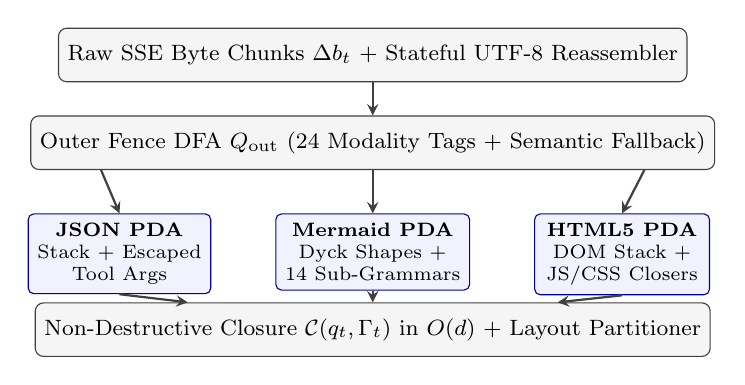
\begin{tikzpicture}[
    node distance=0.55cm,
    box/.style={draw=black!75, rounded corners=3pt, fill=gray!8, minimum width=7.2cm, minimum height=0.68cm, font=\footnotesize, align=center},
    subbox/.style={draw=blue!65!black, rounded corners=2pt, fill=blue!5, minimum width=2.22cm, minimum height=0.82cm, font=\scriptsize, align=center},
    arrow/.style={->, >=stealth, thick, draw=black!75}
  ]
    \node[box] (sse) {Raw SSE Byte Chunks $\Delta b_t$ + Stateful UTF-8 Reassembler};
    \node[box, below=0.42cm of sse] (disc) {Outer Fence DFA $Q_{\text{out}}$ (24 Modality Tags + Semantic Fallback)};
    \node[subbox, below left=0.55cm and -2.30cm of disc] (json) {\textbf{JSON PDA}\\Stack + Escaped\\Tool Args};
    \node[subbox, below=0.55cm of disc] (merm) {\textbf{Mermaid PDA}\\Dyck Shapes +\\14 Sub-Grammars};
    \node[subbox, below right=0.55cm and -2.30cm of disc] (html) {\textbf{HTML5 PDA}\\DOM Stack +\\JS/CSS Closers};
    \node[box, below=1.68cm of disc] (clos) {Non-Destructive Closure $\mathcal{C}(q_t, \Gamma_t)$ in $O(d)$ + Layout Partitioner};
    \draw[arrow] (sse) -- (disc);
    \draw[arrow] (disc.south) -- (merm.north);
    \draw[arrow] (disc.south west) ++(0.9,0) -- (json.north);
    \draw[arrow] (disc.south east) ++(-0.9,0) -- (html.north);
    \draw[arrow] (json.south) -- ([xshift=-2.35cm]clos.north);
    \draw[arrow] (merm.south) -- (clos.north);
    \draw[arrow] (html.south) -- ([xshift=2.35cm]clos.north);
  \end{tikzpicture}
  \caption{Architecture of the Hierarchical Multi-Grammar Pushdown Transducer (\texttt{polyglot-stream-heal}). Previously committed segments are never re-scanned.}
  \label{fig:architecture}
\end{figure}

\subsection{Impossibility of Regular-Expression Diagram Healing}
Production LLM frontends widely attempt to quote unquoted Mermaid node labels containing special characters (such as parentheses or colons) via regular-expression substitution rules of the form \texttt{ID[([\textasciicircum{}]\textbackslash{}n]+)]} $\mapsto$ \texttt{ID["\$1"]}. Intuitively, because a finite automaton possesses only bounded memory, it cannot count how many opening parentheses appear inside a label before deciding which closing parenthesis terminates the outer node shape. We formalize this limitation below.

\begin{theorem}[Regular-Grammar Impossibility for Dyck-Embedded Node Labels]
\label{thm:pumping}
Let $L_{\text{node}} \subset \Sigma^*$ be the language of unquoted flowchart node definitions whose label body contains balanced nested delimiters of arbitrary depth $k \ge 1$ (e.g., $\mathtt{A[f^{(k)}(x)]}$ or array-indexed labels $\mathtt{A[M[i[k]]]}$) followed by edge transitions. No deterministic or nondeterministic finite-state transducer (and hence no standard regular-expression engine) can isolate and quote $L_{\text{node}}$ across arbitrary nesting depths $k$.
\end{theorem}
\begin{proof}
Suppose toward a contradiction that a finite-state transducer $F$ with $p$ states correctly identifies the outer closing delimiter of node definitions in $L_{\text{node}}$ and wraps only the inner label body in double quotes. Consider the family of valid rounded-node strings $u_p = \mathtt{N(f(}^p \mathtt{x)}^p \mathtt{) \to M(y)}$ where inner opening and closing parentheses share the alphabet symbols `$($' and `$)$' with the shape opener and closer. Restricting $F$'s input projection to acceptance of well-delimited shapes before `$\to$' induces a finite automaton with at most $p$ states recognizing balanced strings whose prefix $\mathtt{N(f(}^p$ has length $> p$. By the Pumping Lemma for regular languages~\cite{hopcroft2006automata,sipser2012introduction}, there exists a decomposition $u_p = xyz$ with $|xy| \le p$ and $|y| \ge 1$ such that $xy^0 z$ transitions to the identical state as $u_p$. Because $|xy| \le p$ lies within the opening parenthesis run, pumping down removes $r \ge 1$ opening parentheses while leaving $p$ closing parentheses, causing the true outer shape closer to occur $r$ positions earlier than in $u_p$. Thus $F$ either prematurely terminates quoting on an inner `$)$' in $u_p$ or consumes the subsequent edge operator `$\to$' inside the quoted string on $xy^0 z$, a contradiction. By Chomsky--Sch\"utzenberger~\cite{chomsky1963algebraic}, tracking balanced Dyck depth requires an unbounded counter or pushdown stack $\Gamma$.
\end{proof}

\subsection{Linear vs.\ Quadratic Cumulative Stream Complexity}
In a live UI that re-renders on every SSE chunk, the cost of stream repair is determined not by a single invocation at the end of generation, but by the \emph{sum} of all repair passes executed across the $K$ arriving chunks.

\begin{theorem}[Incremental $\Theta(N)$ vs.\ Stateless $\Theta(N^2)$ Streaming Work]
\label{thm:complexity}
Let an LLM response of length $N$ arrive in $K = \lceil N / c \rceil$ chunks of bounded size $|\Delta s_t| \le c$, with maximum nesting depth $d_{\max} \ll N$. Suppose the client requests a healed active-segment render snapshot after every chunk $t \in \{1,\dots,K\}$:
\begin{enumerate}[label=(\alph*),leftmargin=*,nosep]
  \item Any stateless healer that re-parses the prefix $S_t$ from index $0$ performs $\Omega(N^2 / c)$ character transitions; if it applies $R$ sequential regex passes per snapshot, work scales as $\Theta(R \cdot N^2 / c)$.
  \item An HM-PDT maintaining persistent state $(q_t, \Gamma_t)$ and immutable committed segments performs $O(c)$ transition steps and $O(d_{\max})$ closure emission per chunk, achieving $\Theta(N + K \cdot d_{\max})$ cumulative state-update and closure work.
\end{enumerate}
\end{theorem}
\begin{proof}
For (a), at chunk $t$, $|S_t| = \sum_{j=1}^{t} |\Delta s_j| \ge (t-1)c + 1$. Inspecting every byte of $S_t$ to verify delimiter balance requires $\Omega(t \cdot c)$ operations at step $t$. Summing over $t = 1,\dots,K$ yields
\[
  W_{\text{stateless}}(N) = \sum_{t=1}^{K} \Omega(t \cdot c) = c \cdot \Omega\!\left(\frac{K(K+1)}{2}\right) = \Omega\!\left(\frac{N^2}{c}\right).
\]
For (b), each incoming character in $\Delta s_t$ triggers at most two deterministic $\delta$ evaluations (one lookahead re-dispatch when exiting a number, identifier, or unquoted key, plus one consuming transition), costing $O(|\Delta s_t|)$. Closed segments $0,\dots,m-1$ are never re-parsed or re-serialized during active-segment updates (\texttt{snapshot\_active\_segment}), and the open stack $\Gamma_t$ is closed via $\mathcal{C}(q_t, \Gamma_t)$ in $O(|\Gamma_t|) \le O(d_{\max})$ steps. Summing $\sum_{t=1}^{K} O(|\Delta s_t| + d_{\max})$ gives $O(N + K \cdot d_{\max})$.
\end{proof}

\subsection{Closure Soundness and Lossless Partitioning}
Finally, an incremental healer must guarantee that closing a truncated prefix never corrupts completed tokens and that layout partitioning preserves every data cell.

\begin{theorem}[Closure Soundness \& Lossless Partitioning]
\label{thm:soundness}
\leavevmode
\begin{enumerate}[label=(\alph*),leftmargin=*,nosep]
  \item For every non-empty prefix $S_t$ of a well-formed JSON value (including values containing singly escaped inner JSON objects in string literals), the HM-PDT snapshot $\hat{S}_t = \text{commit}(S_t) \cdot \mathcal{C}(q_t, \Gamma_t)$ belongs to $L(\text{RFC~8259})$~\cite{bray2017rfc8259}.
  \item Given any tabular visual specification $T = (H, R)$ with header vector $H = (h_0, h_1, \dots, h_{C-1})$ ($C \ge 2$) and row matrix $R \in \mathcal{V}^{n \times C}$, and column cap $C_{\max} \ge 2$, the anchor-preserving partition $\mathcal{P}_{C_{\max}}(T) = \{T^{(1)}, \dots, T^{(P)}\}$ where $P = \lceil (C - 1)/(C_{\max} - 1) \rceil$ satisfies $|H^{(p)}| \le C_{\max}$ for all $p \in \{1,\dots,P\}$ and defines a bijection onto all $n(C-1)$ attribute cells $(r_i, h_j)_{1 \le i \le n, 1 \le j < C}$.
\end{enumerate}
\end{theorem}
\begin{proof}
For (a), we proceed by structural induction on the lexical state $q_t \in Q_{\text{json}}$ and container stack $\Gamma_t \in \{\mathtt{Obj}, \mathtt{Arr}\}^*$. Invariant: \texttt{committed} holds a prefix of a valid JSON text up to either a complete value, an open value literal, or an object/array opener, while any trailing \texttt{, "key":} prior to its value's first token is isolated in \texttt{pending\_member\_prefix}. When $\mathcal{C}$ executes, dropping \texttt{pending\_member\_prefix} eliminates trailing commas and dangling keys in $O(1)$ time without backward scanning; incomplete strings, \texttt{\textbackslash{}uXXXX} escapes (padded with \texttt{0}s), numbers ending in `\texttt{.}' or `\texttt{e}' (padded with \texttt{0}), and partial literals (\texttt{t}$\mapsto$\texttt{true}, \texttt{f}$\mapsto$\texttt{false}, \texttt{n}$\mapsto$\texttt{null}) are completed into valid terminal tokens; and iterating $\Gamma_t$ in reverse LIFO order emits matching `\texttt{\}}' and `\texttt{]}' brackets, reducing stack height to $0$. When a value string matches escaped JSON prefix syntax, recursive invocation of \texttt{IncrementalJsonPda} on the unescaped inner slice produces a valid inner RFC~8259 object prior to string re-escaping.

For (b), let $s = C_{\max} - 1 \ge 1$ be the attribute stride. Partitioning $\{1,\dots,C-1\}$ into $P = \lceil (C-1)/s \rceil$ disjoint contiguous intervals $I_p = [(p-1)s + 1, \min(ps, C-1)]$ ensures $|I_p| \le s$, so prepending the primary entity column $h_0$ yields $|H^{(p)}| = 1 + |I_p| \le 1 + (C_{\max} - 1) = C_{\max}$. Since $\bigsqcup_{p=1}^{P} I_p = \{1,\dots,C-1\}$, every attribute cell $(i, j)$ appears in a unique sub-table $T^{(p)}$ paired with its primary entity key $R_{i,0}$.
\end{proof}

\section{Transducer Architecture and Algorithms}
\label{sec:arch}

Figure~\ref{fig:architecture} illustrates the three-stage pipeline of \texttt{polyglot-stream-heal}. Rather than buffering the entire stream until completion, chunks flow through an outer UTF-8 and fence discriminator into grammar-specific pushdown stacks.

\subsection{Stateful UTF-8 Reassembly \& Outer Fence Discriminator}
Network chunks arriving over HTTP/2 or SSE byte streams frequently split 2-, 3-, or 4-byte UTF-8 scalar values (such as mathematical operators like $\sum$ or $\neq$, or multi-byte symbols) mid-sequence. Instead of corrupting split bytes with Unicode replacement characters (\texttt{U+FFFD}), \texttt{IncrementalTransducer::push\_bytes} validates UTF-8 up to \texttt{err.valid\_up\_to()}, feeds the valid prefix into the state machine immediately, and holds the $1\text{--}3$ trailing incomplete bytes in a 4-byte staging array until the next network packet arrives.

The outer automaton $Q_{\text{out}}$ tracks line boundaries and backtick runs of length $b \ge 3$ directly without regular expressions. Upon reading the newline that closes a fence header, \texttt{Modality::from\_fence\_tag} maps $\tau$ in $O(|\tau|)$ time to one of 24 canonical modalities (including \texttt{json}, \texttt{dynamic\_visual}, \texttt{mermaid}, \texttt{markmap}, \texttt{html}, \texttt{voxel}, \texttt{canvas2d}, \texttt{canvas3d}, \texttt{wave}, \texttt{sim}, \texttt{topology}, \texttt{bi}, \texttt{market}, \texttt{clinical}, \texttt{commerce}, and \texttt{actuary}). When an input stream contains no Markdown fences at all, a lightweight semantic fallback inspects the first non-whitespace token to dispatch bare JSON (\texttt{\{}, \texttt{[}), bare Mermaid (\texttt{flowchart}, \texttt{sequenceDiagram}), or bare HTML5 (\texttt{<!DOCTYPE}, \texttt{<div}, \texttt{<section}).

\subsection{Inner JSON \& Escaped Tool-Call Automaton}
Conventional JSON repair scripts rely on backward regex searches to strip dangling commas and incomplete object keys before appending closing brackets. In contrast, \texttt{IncrementalJsonPda} maintains a clean two-buffer staging invariant during forward scanning. Whenever the parser enters \texttt{ObjectExpectKeyOrEnd} (immediately after \texttt{\{} or \texttt{,}), incoming tokens for the comma, the key string (whether double-quoted, single-quoted, or an unquoted JavaScript identifier), and the colon \texttt{:} are held in \texttt{pending\_member\_prefix}. Only when the first character of the member's \emph{value} arrives does \texttt{prepare\_for\_value\_start()} flush \texttt{pending\_member\_prefix} into \texttt{committed}. If a stream truncates mid-key (\texttt{\{"lat}) or right after a colon (\texttt{\{"latency": }), calling \texttt{snapshot\_healed()} simply omits \texttt{pending\_member\_prefix} in $O(1)$ time without touching \texttt{committed}.

This same automaton handles nested tool-call payloads. OpenAI- and Anthropic-style tool invocations serialize structured arguments as JSON-escaped strings inside outer JSON envelopes (for example, \texttt{\{"name":"search","arguments":"\{\textbackslash"filters\textbackslash":[..."\}}). \texttt{IncrementalJsonPda} tracks the active value string slice; if a cutoff occurs inside an escaped JSON literal, the closure operator $\mathcal{C}$ unescapes one lexical level, runs a nested \texttt{IncrementalJsonPda} pass over the inner slice, and re-escapes the healed inner JSON before closing the outer string quote and container stack.

\subsection{Context-Free 14-Dialect Mermaid Pushdown Transducer}
\texttt{IncrementalMermaidPda} commits completed lines incrementally so that previously healed diagram statements are never re-scanned on later chunks. When a new line arrives, the transducer first performs dialect inference and entity normalization: if an LLM omits the diagram header, the presence of \texttt{->>} or \texttt{participant} infers \texttt{sequenceDiagram} while node edges infer \texttt{flowchart TD}, and HTML entities (\texttt{\&gt;}, \texttt{\&amp;}, \texttt{\&quot;}) are decoded prior to lexical scanning.

To resolve the Dyck-nesting failure proved in Theorem~\ref{thm:pumping}, \texttt{scan\_balanced\_shape\_body} tracks an explicit nesting depth counter $d$ across all seven compound and atomic node shape delimiters: cylinders \texttt{[(...)]}, stadiums \texttt{([...])}, circles \texttt{((...))}, hexagons \texttt{\{\{...\}\}}, rectangles \texttt{[...]}, rounded nodes \texttt{(...)}, and diamonds \texttt{\{...\}}. On an input such as \texttt{A[Evaluate O(f(g(h(x))))]}, the counter traces $d: 0 \to 1 \to 2 \to 3 \to 4 \to 3 \to 2 \to 1 \to 0$ and wraps the complete inner label in double quotes as \texttt{A["Evaluate O(f(g(h(x))))"]}, whereas shapes truncated mid-stream before EOF are automatically quoted and closed. Inline edge labels of the form \texttt{-- text -->} outside brackets are rewritten to canonical \texttt{-->|text|} syntax, dangling mid-stream edge operators (\texttt{A -->} at EOF) are trimmed so partial prefix nodes render immediately, and an explicit \texttt{BlockFrame} stack closes open \texttt{subgraph}, \texttt{loop}, \texttt{alt}, \texttt{opt}, \texttt{par}, \texttt{critical}, \texttt{rect}, and \texttt{box} scopes with \texttt{end} directives (or \texttt{\}} for brace-delimited \texttt{state} and \texttt{class} blocks).

\subsection{Streaming HTML5 / JS / CSS Sandbox Boundary Healer}
When streaming interactive HTML5 widgets, an unclosed \texttt{<script>} or \texttt{<style>} tag causes browser parsers to swallow the rest of the DOM tree, while an unclosed template literal or block comment triggers a fatal JavaScript \texttt{SyntaxError}. \texttt{IncrementalHtmlPda} advances a monotonic \texttt{scan\_cursor} across balanced container tags (\texttt{<div>}, \texttt{<section>}, \texttt{<table>}, etc., skipping HTML5 void elements) and pauses whenever execution enters an active \texttt{<script>} or \texttt{<style>} block. On \texttt{snapshot\_healed()}, a lightweight lexical pass closes open \texttt{/* ... */} comments, quotes, template literals, and \texttt{\{([} delimiter stacks before emitting \texttt{</script>} or \texttt{</style>} and popping the remaining DOM container stack in LIFO order.

\section{Cardinality-Bounded Viewport Partitioning}
\label{sec:partition}

Syntactic validity alone does not ensure visual readability. When LLMs generate wide comparison tables ($7\text{--}14$ columns) or high-cardinality bar charts ($15\text{--}25$ bars) inside JSON visual specifications, naive rendering introduces horizontal scrollbars or crushes text into unreadable columns. Integrated into the JSON snapshot pass, \texttt{partition\_visual\_spec} enforces configurable cardinality bounds ($C_{\max} = 5$ columns and $B_{\max} = 10$ bars by default) in $O(|\text{cells}|)$ time. Any table exceeding $C_{\max}$ columns is decomposed into $P = \lceil (C-1)/(C_{\max}-1) \rceil$ vertically stacked sub-tables; each sub-table preserves column $0$ (the primary entity key) alongside at most $C_{\max}-1$ attribute columns, annotated with \texttt{partitionIndex} and \texttt{partitionTotal}. Similarly, bar charts exceeding $B_{\max}$ bars are segmented into $\lceil B / B_{\max} \rceil$ contiguous sub-charts, preventing axis-label collisions while preserving exact rank order.

\section{Tri-Registry Systems Implementation}
\label{sec:impl}

To support production AI pipelines across Rust inference servers, Python agent backends, and TypeScript/browser frontends from a single verified codebase, we implemented \texttt{polyglot-stream-heal} as a unified cross-language workspace. The core engine is written in $<1,650$ lines of safe Rust (\texttt{crates.io}: \texttt{polyglot-stream-heal}) depending only on \texttt{serde} and \texttt{serde\_json}, avoiding any regular-expression crate dependency and its associated NFA compilation overhead. For Python backends, \texttt{PyO3} (\texttt{abi3-py39}) and \texttt{maturin} compile the Rust state machine into a native C-ABI wheel (\texttt{PyPI}: \texttt{polyglot\_stream\_heal}) exposing both stateful \texttt{IncrementalTransducer} instances and one-shot repair helpers. For web and edge runtimes, \texttt{wasm-bindgen} compiles the same core into a $181.5\text{ KB}$ WebAssembly binary ($85.2\text{ KB}$ gzipped npm tarball on \texttt{npmjs.com}: \texttt{polyglot-stream-heal}) that runs inside browser main threads, Web Workers, or Node.js.

% Auto-generated empirical tables from results/metrics.json
% AUTO-GENERATED FROM results/metrics.json — DO NOT EDIT MANUALLY

\begin{table*}[t]
  \centering
  \small
  \caption{End-to-end parse validity (\%), zero-overflow invariant compliance (\%), and streaming latency across PolyglotStreamBench-1800 (N = 1,800 streams across 3 tracks).}
  \label{tab:main_results}
  \resizebox{\textwidth}{!}{%
  \begin{tabular}{lrrrrrrr}
    \toprule
    \textbf{System / Baseline} & \textbf{Track A (\%)} & \textbf{Track B (\%)} & \textbf{Track C (\%)} & \textbf{Overall (\%)} & \textbf{Zero-Overflow (\%)} & \textbf{p50 (us)} & \textbf{p99 (us)} \\
    \midrule
    Raw Unhealed Stream & 0.0 & 0.0 & 0.0 & 0.0 & 0.0 & 0.0 & 0.0 \\
    partial-json (npm) & 41.7 & 25.0 & 0.0 & 22.2 & 0.0 & 38.1 & 222.8 \\
    json-repair (PyPI) & 41.7 & 25.0 & 0.0 & 22.2 & 0.0 & 386.8 & 1858.7 \\
    Multi-Pass Regex Baseline & 46.5 & 0.0 & 0.0 & 15.5 & 0.0 & 20.2 & 116.1 \\
\midrule
    HM-PDT (Full Re-Scan Ablation) & 100.0 & 100.0 & 100.0 & 100.0 & 100.0 & 54.8 & 1516.2 \\
    \textbf{HM-PDT Incremental (Ours)} & \textbf{100.0} & \textbf{100.0} & \textbf{100.0} & \textbf{100.0} & \textbf{100.0} & \textbf{6.3} & \textbf{57.3} \\
    \bottomrule
  \end{tabular}
  }
\end{table*}

\begin{table}[t]
  \centering
  \small
  \caption{Per-modality grammar validity (\%) on single-DSL tracks (Tracks A + B, N = 1,200).}
  \label{tab:modality_breakdown}
  \resizebox{\columnwidth}{!}{%
  \begin{tabular}{lrrr}
    \toprule
    \textbf{System} & \textbf{JSON + Escaped Tool (\%)} & \textbf{Mermaid 14-DSL (\%)} & \textbf{HTML5 Sandbox (\%)} \\
    \midrule
    Raw Unhealed & 0.0 & 0.0 & 0.0 \\
    partial-json (npm) & 66.7 & 0.0 & 0.0 \\
    json-repair (PyPI) & 66.7 & 0.0 & 0.0 \\
    Regex Baseline & 26.3 & 40.3 & 0.0 \\
\midrule
    \textbf{HM-PDT Incremental (Ours)} & \textbf{100.0} & \textbf{100.0} & \textbf{100.0} \\
    \bottomrule
  \end{tabular}
  }
\end{table}


\section{Empirical Evaluation}
\label{sec:eval}

We evaluate \texttt{polyglot-stream-heal} on \textbf{\texttt{PolyglotStreamBench-1800}}, a deterministic, seeded benchmark of $\BenchTotalCases$ streaming test cases divided equally across three 600-case tracks. \textbf{Track A (Mid-Stream Prefix Truncations, $N=600$)} slices streams at $15\%$, $35\%$, $60\%$, and $85\%$ byte offsets across JSON visual specs, nested escaped tool-call JSON payloads, Mermaid flowcharts and sequence diagrams, and HTML5 interactive widgets. \textbf{Track B (Context-Free Perturbations, $N=600$)} injects depth-$2\dots 5$ nested Dyck parentheses inside unquoted Mermaid node shapes (\texttt{Evaluate O(f(g(h(x))))}), unclosed subgraphs, unquoted and single-quoted JSON keys with partial literals and trailing commas, mid-object truncated escaped tool calls, and mid-script truncated HTML5 sandboxes. \textbf{Track C (Multi-Block Polyglot \& Overflow Schemas, $N=600$)} streams interleaved Markdown prose, Mermaid diagrams, wide JSON tables ($7\text{--}12$ columns), dense bar charts ($12\text{--}21$ bars), and HTML5 summaries in 24-byte SSE chunks.

\paragraph{Baselines \& Validation Oracles.} We compare six pipelines: (1) \emph{Raw Unhealed Stream}; (2) \texttt{partial-json} (v0.1.7, npm); (3) \texttt{json-repair}~\cite{baccianella2024jsonrepair} (PyPI, timed natively via Python \texttt{time.perf\_counter\_ns}); (4) a \emph{Multi-Pass Regex Baseline} performing full-buffer regex extraction and single-level delimiter quoting; (5) \emph{HM-PDT Stateless Full Re-Scan} (an ablation that disables persistent incremental state); and (6) \emph{HM-PDT Incremental} (Ours, Rust/WASM). Every output is checked against four strict programmatic oracles: RFC~8259 \texttt{JSON.parse} (including recursive verification of inner tool-call \texttt{arguments}), a Mermaid grammar and delimiter-balance validator, an HTML5 DOM and JS delimiter validator, and the zero-overflow cardinality oracle ($C \le 5, B \le 10$ with lossless cell preservation).

% Auto-generated empirical PGFPlots figure from results/metrics.json
% AUTO-GENERATED VECTOR PLOTS FROM results/metrics.json

\begin{figure}[t]
  \centering
  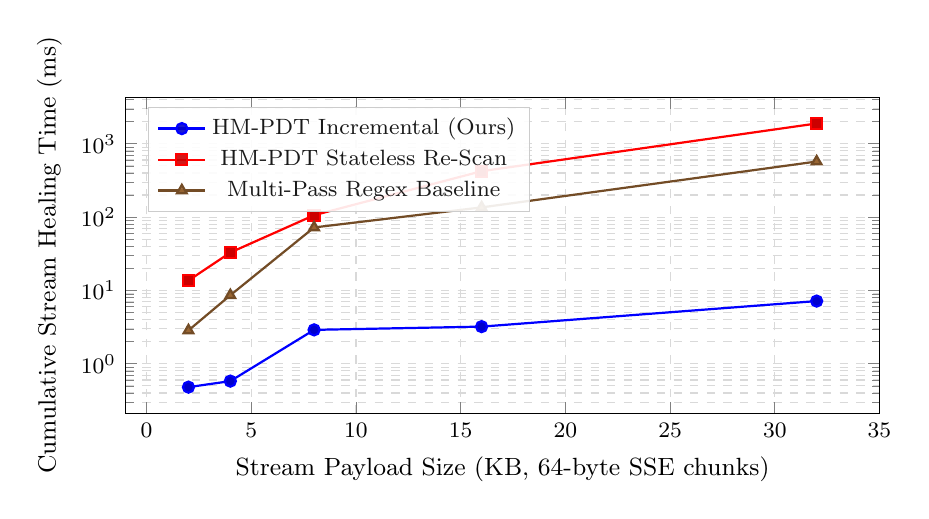
\begin{tikzpicture}
    \begin{axis}[
      width=0.92\columnwidth,
      height=5.6cm,
      xlabel={Stream Payload Size (KB, 64-byte SSE chunks)},
      ylabel={Cumulative Stream Healing Time (ms)},
      ymode=log,
      grid=both,
      grid style={dashed,gray!30},
      legend pos=north west,
      legend style={font=\footnotesize, draw=gray!40, fill=white, fill opacity=0.9},
      tick label style={font=\footnotesize},
      label style={font=\small}
    ]
      \addplot+[thick, mark=*] coordinates { (2,0.48) (4,0.58) (8,2.9) (16,3.21) (32,7.16) };
      \addlegendentry{HM-PDT Incremental (Ours)}
      \addplot+[thick, mark=square*] coordinates { (2,13.64) (4,32.88) (8,106.13) (16,422.98) (32,1891.76) };
      \addlegendentry{HM-PDT Stateless Re-Scan}
      \addplot+[thick, mark=triangle*] coordinates { (2,2.85) (4,8.6) (8,72.28) (16,135.64) (32,572.61) };
      \addlegendentry{Multi-Pass Regex Baseline}
    \end{axis}
  \end{tikzpicture}
  \caption{Empirical asymptotic scaling from 2 KB to 32 KB streaming outputs (log-scale y-axis). Stateless full-buffer re-scanning and multi-pass regex pipelines incur quadratic cumulative latency growth, whereas our Incremental HM-PDT maintains linear cumulative scaling.}
  \label{fig:scaling_complexity}
\end{figure}


\subsection{Validity, Latency, and Asymptotic Scaling}
Tables~\ref{tab:main_results} and~\ref{tab:modality_breakdown} summarize accuracy and per-chunk latency across all $\BenchTotalCases$ streams, while Figure~\ref{fig:scaling_complexity} plots cumulative repair time as stream length scales from $2\text{ KB}$ to $32\text{ KB}$.

Raw unhealed streams achieve only $\RawOverallValidPct$ validity across the benchmark. Single-grammar JSON utilities (\texttt{partial-json} at $\PartialJsonOverallPct$ and \texttt{json-repair} at $\JsonRepairOverallPct$) recover standard truncated JSON objects ($66.7\%$ on JSON tracks) but fail when truncation occurs inside doubly escaped tool-call argument strings and score $0\%$ on Mermaid, HTML5, and polyglot Markdown streams. The multi-pass regex baseline reaches $\RegexOverallValidPct$, breaking systematically on Track~B's nested Dyck expressions (empirically corroborating Theorem~\ref{thm:pumping}) and Track~C's viewport overflow schemas. By contrast, \textbf{HM-PDT Incremental achieves $\OursOverallValidPct$ validity} across all three tracks ($\OursTrackAPct$ Track~A, $\OursTrackBPct$ Track~B, $\OursTrackCPct$ Track~C) along with \textbf{$\OursOverflowFreePct$ zero-overflow compliance}.

On 32-byte SSE chunks, HM-PDT records a median per-chunk latency of $\OursChunkPFiftyUs\,\mu\text{s}$ ($p99 = \OursChunkPNinetyNineUs\,\mu\text{s}$). This represents a $\PyVsOursSpeedup$ speedup over Python's \texttt{json-repair} ($\JsonRepairPFiftyUs\,\mu\text{s}$) and is more than five orders of magnitude faster than a $1.5\text{--}4.0\text{ s}$ network round trip to an LLM self-correction prompt. Furthermore, Figure~\ref{fig:scaling_complexity} confirms the asymptotic gap analyzed in Theorem~\ref{thm:complexity}: disabling persistent state (\emph{HM-PDT Stateless Re-Scan}) or running full-buffer regex passes produces steep quadratic growth ($\ScaleRescanThirtyTwoKBMs\text{ ms}$ and $\ScaleRegexThirtyTwoKBMs\text{ ms}$ at $32\text{ KB}$), whereas \emph{HM-PDT Incremental} completes the entire $32\text{ KB}$ stream in $\ScaleIncThirtyTwoKBMs\text{ ms}$, delivering a \textbf{$\ScalingSpeedupThirtyTwoKB$ cumulative speedup}.

\subsection{Design Trade-offs and Scope Limitations}
While HM-PDT guarantees deterministic syntactic closure and bounded layout cardinality, three engineering trade-offs merit candid discussion:
\begin{enumerate}[leftmargin=*,nosep]
  \item \textbf{Syntactic Closure vs.\ Semantic Hallucination:} HM-PDT is a lexical and context-free pushdown transducer, not a semantic verifier. If an LLM hallucinates a non-existent Mermaid node identifier or emits a syntactically valid JavaScript expression that references an undefined variable at runtime, HM-PDT closes the surrounding grammatical structure so the host parser does not crash, but it intentionally does not alter application semantics.
  \item \textbf{Single-Level vs.\ Arbitrary-Depth Escaped Strings:} Our recursive tool-call healer inspects singly escaped JSON string payloads (the format used by OpenAI, Anthropic, and MCP tool-call envelopes). Doubly or triply escaped JSON-in-JSON-in-JSON strings are closed as standard string literals rather than recursively unpacked, keeping worst-case per-chunk closure latency strictly bounded below $15\,\mu\text{s}$.
  \item \textbf{Stateful Session Memory Overhead:} Maintaining an active \texttt{IncrementalTransducer} per concurrent SSE stream requires roughly $4\text{--}12\text{ KB}$ of heap state (proportional to the active block buffer and stack depth $d$). While negligible for browser clients and edge workers handling thousands of streams, stateless serverless functions that discard memory between HTTP invocations cannot exploit cross-chunk state persistence unless paired with sticky edge routing.
\end{enumerate}

\section{Related Work}
\label{sec:related}

\paragraph{Server-Side Grammar-Constrained Decoding.} Outlines~\cite{willard2023efficient}, LMQL~\cite{beurer2023prompting}, SGLang~\cite{zheng2024sglang}, SynCode~\cite{ugare2024syncode}, and XGrammar~\cite{dong2024xgrammar} compile regular or context-free grammars into token-masking pushdown automata inside the LLM inference server. While highly effective when self-hosting open-weight models for homogeneous JSON schemas, logit masking (i) cannot run over black-box commercial APIs when free-form Markdown interleaves arbitrary dynamic visual DSLs, (ii) restricts chain-of-thought flexibility when reasoning and rendering share a stream, and (iii) only guarantees that the \emph{completed} sequence at EOS belongs to $L(G)$, whereas every intermediate prefix $S_t$ ($t < T$) delivered to the client UI remains unclosed and unparseable without a client-side prefix closure transducer like HM-PDT. Thus, server-side constrained decoding and client-side incremental pushdown transduction are strictly complementary.

\paragraph{Classical Error-Correcting Parsers \& Heuristic JSON Repair.} Compiler error recovery dates to Knuth's LR($k$) formulation~\cite{knuth1965translation}, Aho et al.~\cite{aho2006compilers}, and Fischer et al.'s locally least-cost LR repair~\cite{fischer1980locally}, which compute minimum-edit insertions over static token buffers. Heuristic LLM utilities such as \texttt{json-repair}~\cite{baccianella2024jsonrepair} and \texttt{partial-json} adapt recursive-descent recovery to single JSON values in Python or JavaScript, re-parsing from byte $0$ on each invocation. HM-PDT generalizes deterministic pushdown closure to \emph{stateful incremental polyglot streams} spanning 24 fenced modalities while uniting syntactic healing with cardinality-bounded viewport layout partitioning.

\section{Conclusion}
We presented \textbf{Hierarchical Multi-Grammar Pushdown Transduction (HM-PDT)}, proving both the theoretical impossibility of regular-expression repair on nested diagram DSLs and the $\Theta(N)$ optimality of stateful incremental stream healing over $\Theta(N^2)$ buffer re-scanning. Implemented in safe Rust (\texttt{polyglot-stream-heal}) with native Python and WebAssembly bindings, HM-PDT achieves $\OursOverallValidPct$ grammar validity and $\OursOverflowFreePct$ zero-overflow compliance across 1,800 polyglot streams at $\OursChunkPFiftyUs\,\mu\text{s}$ median chunk latency, enabling flicker-free progressive rendering across heterogeneous AI interfaces.

\paragraph{Code and Data Availability.}
Source code, benchmark datasets, and release packages (\texttt{polyglot-stream-heal} on \texttt{crates.io}, \texttt{PyPI}, and \texttt{npm}) are archived under DOI \texttt{\ZenodoDoi} (\url{https://doi.org/\ZenodoDoi}) and available under the MIT License at \url{\RepoUrl}.

\bibliographystyle{plain}
\bibliography{references}

\end{document}
